\documentclass{article}

\usepackage[T2A]{fontenc}
\usepackage[utf8]{inputenc}
\usepackage[russian, english]{babel}
\usepackage[left=2.3cm, right=2.3cm, top=2.7cm, bottom=2.7cm, bindingoffset=0cm, margin=3in]{geometry}
\parindent 0pt
\parskip -5pt
\usepackage{amsmath}
\usepackage{amssymb}
\usepackage{amsfonts}
\usepackage{amsthm}
\usepackage{graphicx}
\usepackage[shortlabels]{enumitem}
\usepackage[all]{xy}
\usepackage[usenames]{color}
\linespread{1.5}


\usepackage{color}
\usepackage{listings}
\definecolor{mygreen}{rgb}{0,0.6,0}
\definecolor{mygray}{rgb}{0.5,0.5,0.5}
\definecolor{mymauve}{rgb}{0.58,0,0.82}
\definecolor{myorange}{rgb}{0.855,0.576,0.027}
\lstset{
    language=Octave,
    basicstyle=\ttfamily,
    frame=tb,
    extendedchars=\true,
    morecomment = [l][\itshape\color{blue}]{\%},
    keywordstyle=\color{blue},
    commentstyle=\color{mygreen},
    breakatwhitespace=false,         
    breaklines=true,  
    numbers=left,
    numbersep=-10pt,
    numberstyle=\tiny\color{mygray}, 
    showstringspaces=false,
    showtabs=false,                  
    tabsize=4,
    stringstyle=\color{myorange},
    title=\lstname,
    literate=
    {+}{{{\color{red}+}}}1
    {-}{{{\color{red}-}}}1
    {*}{{{\color{red}*}}}1
    {,}{{{\color{red},}}}1
    {=}{{{\color{red}=}}}1
    {)}{{{\color{red})}}}1
    {(}{{{\color{red}(}}}1
    {;}{{{\color{red};}}}1
    {:}{{{\color{red}:}}}1
    {[}{{{\color{red}[}}}1
    {]}{{{\color{red}]}}}1
    {>}{{{\color{red}>}}}1
}


\title{\textbf{Отчёт №8 (вар.14)} Оценка квадратичной и линейной функции методом наименьших
квадратов}
\author{Романенко Демьян, М3238\\
    \texttt{romanenko@niuitmo.ru}}
\date{18.06.2020}

\begin{document}

    \pagenumbering{gobble}
	\maketitle
	\newpage
	\newgeometry{margin=0.8in}
	\pagenumbering{arabic}
    
    \maketitle
    
    \section{Постановка задачи}
        \begin{enumerate}
            \item Квадратичная функция \begin{itemize}
                \item Смоделировать квадратичную функцию $y(x) = \alpha_1 x^2 + \alpha_2 x + \alpha_3$, наблюдаемую в нормальных шумах в пакете Octave в соответствии с параметрами варианта;
                \item Оценить коэффициенты квадратичной зависимости, уровень шумов и квадратичную функцию по зашумленным данным;
                \item Сравнить полученные результаты с "истинными" данными.
            \end{itemize}
            \item Линейная функция \begin{itemize}
                \item Смоделировать линейную функцию $y(x) = c_1 x + c_2$, наблюдаемую в нормальных шумах в пакете Octave в соответствии с параметрами варианта;
                \item Оценить коэффициенты линейной зависимости, уровень шумов и линейную функцию по зашумленным данным;
                \item Построить доверительный интервал для значений функции при уровне доверия 0.95;
                \item Сравнить полученные результаты с "истинными" данными.
            \end{itemize}
        \end{enumerate}
    \paragraph{Исходные данные}
        \begin{enumerate}
            \item $x_{min} = -2.2$, $x_{max} = 2.5$ {---} границы интервала;
            \item $n = 69$ {---} число точек;
            \item $a_1 = 1.7$, $a_2 = -2.4$, $a_3 = -3.6$ {---} коэффициенты квадратичной функции;
            \item $c_1 = 3.5$, $c_2 = -4.2$ {---} коэффициенты линейной функции;
            \item $s = 1.5$ {---} уровень шумов.
        \end{enumerate}    
    \section{Исходный код программ}
    \subsection{Квадратичная функция}
        \begin{lstlisting}[caption={quad.m}]
    pkg load statistics;
    
    clc;
    clear;

    x_min = -2.2; 
    x_max = 2.5;
    n = 69;
    a = [1.7, -2.4, -3.6];
    s = 1.5;

    X = (x_min : (x_max - x_min) / (n - 1) : x_max)';
    y = polyval(a, X);

    Z = s * randn(n, 1); 
    Y = y + Z;
    plot(X, y, X, Y, '+');

    m = 2;
    an = polyfit(X, Y, m);
    Yn = polyval(an, X);
    plot(X, Y, '+', X, y, X, Yn, 'o');

    e = Yn - Y;
    printf("Actual coefficients a1 = %d, a2 = %d, a3 = %d;\n", a);
    printf("Approximated coefficients: %d, %d, %d;\n", an);
    printf("Scalar product e and Yn: %d;\n", e' * Yn);
    printf("Noise(s) = %d; Noise(sn) = %d.\n", s, sqrt(e' * e / (n - 2)));
        \end{lstlisting}        
    \subsection{Линейная функция}
        \begin{lstlisting}[caption={linear.m}]
    pkg load statistics;
        
    clc;
    clear;
    
    x_min = -2.2;
    x_max = 2.5;
    n = 69;
    c = [3.5, -4.2];
    s = 1.5;
    
    X = (x_min : (x_max - x_min) / (n - 1) : x_max)';
    y = polyval(c, X);
    
    Z = s * randn(n,1); 
    Y = y + Z;
    plot(X, y, X, Y);
    
    % linear regression
    xn = mean(X);
    yn = mean(Y); 
    cov = (X - xn)' * (Y - yn) / (n - 1);
    b = cov / (std(X) ^ 2);
    Yn = yn + b * (X - xn);
    
    % matlab interpolation
    m = 1;
    cn = polyfit(X, Y, m);
    Ynn = polyval(cn, X);
    plot(X, Y, '+', X, y, X, Yn, X, Ynn, 'o');
    
    e = Yn - Y;
    sn = sqrt(e' * e / (n - 2));
    
    ta = 1.96;
    ha = ta * (sn / sqrt(n));
    da = ha * (1 + (X - xn) .^ 2 / (std(X) ^ 2)) .^ (1 / 2);
    Yn1 = Yn - da;
    Yn2 = Yn + da;
    plot(X, Yn1, X, Yn2, X, Y, 'o', X, Yn)
    
    printf("Actual coefficients c1 = %d, c2 = %d;\n", c);
    printf("Approximated coefficients: %d, %d;\n", cn);
    printf("Matlab coefficients: %d, %d;\n", b, yn - b * xn); 
    printf("Scalar product e and Yn: %d;\n", e' * Yn);
    printf("Noise(s) = %d; Noise(sn) = %d.\n", s, sn);
        \end{lstlisting}        
    \newpage    
    \section{Результаты работы программ} 
    \subsection{Квадратичная функция}
        \begin{verbatim}
Actual coefficients a1 = 1.7, a2 = -2.4, a3 = -3.6;
Approximated coefficients: 1.69016, -2.25855, -3.57421;
Scalar product e and Yn: 3.57492e-14;
Noise(s) = 1.5; Noise(sn) = 1.48824.        
        \end{verbatim}
        \begin{figure}[h]
            \center{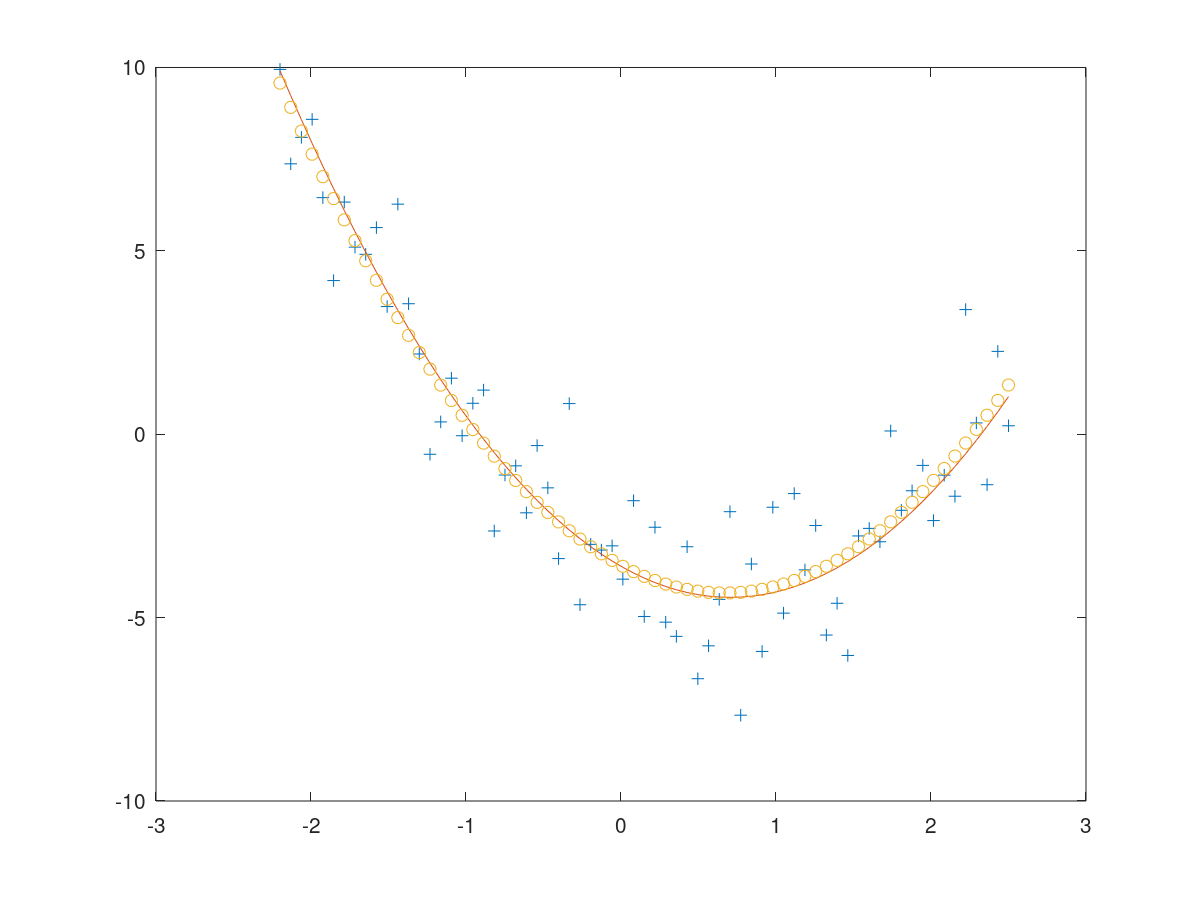
\includegraphics[width=1\linewidth]{quad.png}}
        \end{figure} 
    \newpage    
    \subsection{Линейная функция}
        \begin{verbatim}
Actual coefficients c1 = 3.5, c2 = -4.2;
Approximated coefficients: 3.52776, -4.28172;
Matlab coefficients: 3.52776, -4.28172;
Scalar product e and Yn: 4.70735e-13;
Noise(s) = 1.5; Noise(sn) = 1.29854.
        \end{verbatim}
        \begin{figure}[h]
            \center{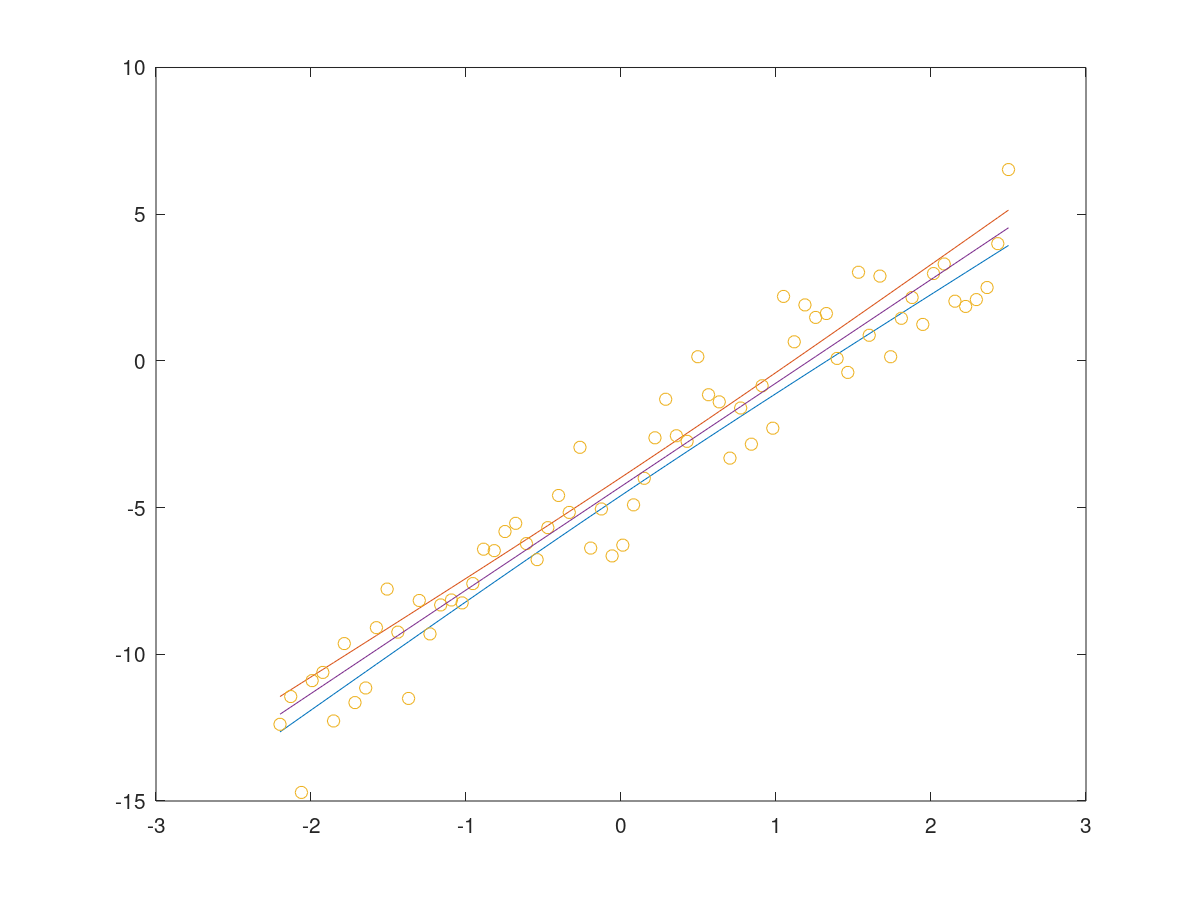
\includegraphics[width=1\linewidth]{linear.png}}
        \end{figure} 
    \section{Вывод}
        Полученная функция попадает в доверительный интервал. Для обеих функций посчитанные коэффициенты близки к исходным. Вектор несвязок практически ортогонален вектору значений зашумлённой функции. Посчитанный уровень шумов близок к теоретическому.
\end{document}
